\documentclass[a4paper]{article}
\usepackage{interspeech2013,amssymb,amsmath,epsfig}
\setcounter{page}{1}
\sloppy		% better line breaks
\ninept
%SM below a registered trademark definition
\def\reg{{\rm\ooalign{\hfil
     \raise.07ex\hbox{\scriptsize R}\hfil\crcr\mathhexbox20D}}}

%% \newcommand{\reg}{\textsuperscript{\textcircled{\textsc r}}}
\title{Relationships Between Prosodic-Linguistic Features and High-Level Descriptors of Speed Dates}

%%%%%%%%%%%%%%%%%%%%%%%%%%%%%%%%%%%%%%%%%%%%%%%%%%%%%%%%%%%%%%%%%%%%%%%%%%
%% If multiple authors, uncomment and edit the lines shown below.       %%
%% Note that each line must be emphasized {\em } by itself.             %%
%% (by Stephen Martucci, author of spconf.sty).                         %%
%%%%%%%%%%%%%%%%%%%%%%%%%%%%%%%%%%%%%%%%%%%%%%%%%%%%%%%%%%%%%%%%%%%%%%%%%%
%\makeatletter
%\def\name#1{\gdef\@name{#1\\}}
%\makeatother
%\name{{\em Firstname1 Lastname1, Firstname2 Lastname2, Firstname3 Lastname3,}\\
%      {\em Firstname4 Lastname4, Firstname5 Lastname5, Firstname6 Lastname6,
%      Firstname7 Lastname7}}
%%%%%%%%%%%%%%% End of required multiple authors changes %%%%%%%%%%%%%%%%%

\makeatletter
\def\name#1{\gdef\@name{#1\\}}
\makeatother
\name{{\em Sidd Jagadish, Ranjay Krishna, Gabriele Carotti-Sha}}

\address{$^1$Department of Statistics, Stanford University \\
  $^2$Department of Computer Science, Stanford University\\
  $^3$ Symbolic Systems, Stanford University\\
{\small \tt siddj@stanford.edu, rak248@stanford.edu, gcarotti@stanford.edu}}

%
\begin{document}
\maketitle
%

\begin{abstract}
We extract lexical and prosodic features of speech from 1493 speed dates at Stanford University.  Each speed date is accompanied by information about what each participant thought of the other, including 1-10 assessments of courteousness and funniness.  Here, we investigate prediction of these assessments from lexical and prosodic features.  We find that for many labels, lexical and prosodic features can powerfully predict our high-level descriptors.
\end{abstract}

\noindent{\bf Index Terms}: Prosody, Speed Date, AdaBoost, Gender differences in prosody, factor analysis, courteous, funny

%

\section{Introduction}
This template can be found on the conference website. Please use
either a LibreOffice, MS-Word\reg\ or a \LaTeX\ format file when preparing your
submission. Information for full paper submission is available on the
conference web site.

\section{Data}
We were given, courtesy of Jurafsky (2013), a dataset consisting of 1980 (CHECK THIS VALUE) heterosexual speed dates. For each date, we have two .wav files corresponding to the microphones attached to each participant.  We also have high-level descriptors of each participant, including their height, weight, and ethnicity.  In addition to this, for each participant, we have 1-10 assessments of various qualities of both themselves and each other person they went on a speeddate with, including funniness and courteousness.

\subsection{Feature Extraction}
Prosodic features were extracted using openSMILE.  Lexical features were extracted in Python, with the help of the LIWC dictionary.  

\section{Exploratory Analysis}
Before attempting to classify speakers as funny or not, we examine the underlying dimensions along which the data varies.  To do, so we use exploratory factor analysis. To determine the number of factors, we use a scree test and various non-graphical measures, including parallel analysis and an optimal coordinates test, as described in (CITE).  We find an optimal number of factors $k = 5$ for both males and females, conducted separately.  Figure 1 shows the two scree plots.

\begin{figure}[t]
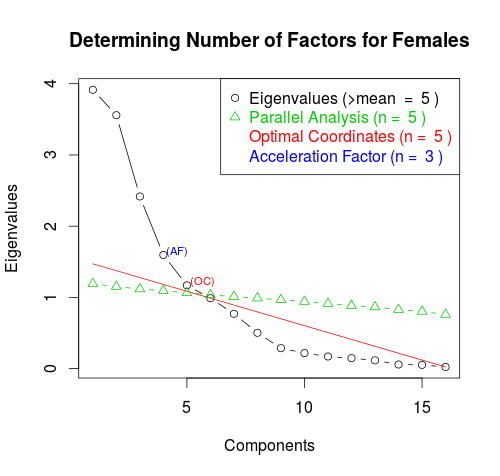
\includegraphics[width = 3.5cm]{graphics/ScreeFem.png}
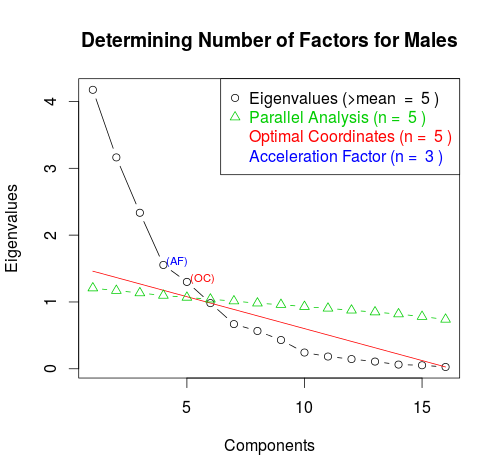
\includegraphics[width = 3.5cm]{graphics/ScreeMale.png}
\caption{{\it Determining Number of Factors}}  
\end{figure}

Interestingly, although we find that the various factors for male and female speech are similar, they explain different amounts of variation in the data.  For males, the first factor reflects high intensity values and low intensity variation, explaining   

\section{Page layout and style}

Authors should observe the following rules for page layout. A
highly recommended way to meet these requirements is to use a given
template (LibreOffice, Word\reg\ or \LaTeX) and check details against the
corresponding example file.

\subsection{Basic layout features}

\begin{itemize}
%\itemsep -1.3mm
\item Proceedings will be printed in A4 format. Authors must submit their papers
in A4 format.
\item Two columns are used except for the title part and possibly for large 
figures that need a full page width.
\item Left margin is 20 mm.
\item Column width is 80 mm.
\item Spacing between columns is 10 mm.
\item Top margin 25 mm (except for the first page which is 30 mm to the title top).
\item Text height (without headers and footers) is maximum 235 mm.
\item Headers and footers must be left empty (they will be added for 
printing and the INTERSPEECH 2013 media).
\item Check indentations and spacings by comparing to this 
example file (in pdf).
\end{itemize}


\subsubsection{Headings}

Section headings are centered in boldface
with the first word capitalized and the rest of the heading in 
lower case. Sub-headings appear like major headings, except they 
start at the left margin in the column.
Sub-sub-headings appear like sub-headings, except they are in italics 
and not boldface. See the examples given in this 
file. No more than 3 levels of headings should be used.

\subsection{Text font}

Times or Times Roman font is used for the main text. Font size in the main text 
must be 9 points, and in the References section 8 points. Other font
types may be used if needed for special purposes. It is VERY IMPORTANT
that while making the final PDF file, you embed all used fonts!

\LaTeX\ users: users should use Adobe Type 1 fonts such as Times or Times
Roman. These are used automatically by the interspeech2013.sty style
file. Authors must not use Type 3 (bitmap) fonts.

\subsection{Figures}

All figures must be centered on the column (or page, if the figure spans 
both columns).
Figure captions should follow each figure and have the format given in 
Figure~\ref{spprod}.

Figures should preferably be line drawings. If they contain gray 
levels or colors, they should be checked to print well on a 
high-quality non-color laser printer.

Graphics (i.e. illustrations, figures) must not use stipple fill
patterns because they will not reproduce properly in Acrobat PDF.
Please use only SOLID FILL COLORS.

Figures which span 2 columns (i.e. occupy full page width) should be
placed at the top or bottom of the page.



\subsection{Tables}

An example of a table is shown as Table \ref{table1}. Somewhat 
different styles are allowed according to the type and purpose of the 
table. The caption text may be above or below the table.

\begin{table} [t,h]
\caption{\label{table1} {\it This is an example of a table.}}
\vspace{2mm}
\centerline{
\begin{tabular}{|c|c|}
\hline
ratio & decibels \\
\hline  \hline
1/1 & 0 \\
2/1 & $\approx 6$ \\
3.16 & 10 \\
10/1 & 20 \\ 
1/10 & -20 \\
100/1 & 40 \\
1000/1 & 60 \\
\hline
\end{tabular}}
\end{table}

\subsection{Equations}

Equations should be placed on separate lines and numbered. Examples 
of equations are given below.
Particularly,
%
%\vspace{-3mm}
\begin{equation}
x(t) = s(f_\omega(t))
\label{eq1}
\end{equation}
where \(f_\omega(t)\) is a special warping function
\begin{equation}
f_\omega(t)=\frac{1}{2\pi j}\oint_C \frac{\nu^{-1k}d\nu}
{(1-\beta\nu^{-1})(\nu^{-1}-\beta)}
\label{eq2}
\end{equation}
A residue theorem states that
\begin{equation}
\oint_C F(z)dz=2 \pi j \sum_k Res[F(z),p_k]
\label{eq3}
\end{equation}
Applying (\ref{eq3}) to (\ref{eq1}), 
it is straightforward to see that
\begin{equation}
1 + 1 = \pi
\label{eq4}
\end{equation}

Finally we have proven the secret theorem of all speech sciences. 
No more math is needed to show how useful the result is! 

\begin{figure}[t]
\centerline{\epsfig{figure=figure,width=80mm}}
\caption{{\it Schematic diagram of speech production.}}  
\label{spprod}
\end{figure}

\subsection{Hyperlinks}

For technical reasons, the proceedings editor will strip all active
links from the papers during processing. Hyperlinks can be included in
your paper, if written in full, eg. ``http://www.foo.com/index.html''.
The link text must be all black. Please make sure that they present no
problems in printing to paper.

\subsection{Multimedia files}

The INTERSPEECH 2013 organizing committee offers the possibility to submit
multimedia files. These files are meant for audio-visual illustrations that
cannot be conveyed in text, tables and graphs. Just like you would when
including graphics, make sure that you have sufficient author rights to the
multimedia materials that you submit for publication. The proceeding media
will NOT contain readers or players, so be sure to use widely accepted file
formats, such as MPEG, Windows WAVE PCM (.wav) or Windows Media Video
(.wmv) using standard codecs. The files you submit will be accessible from
the abstract cards on the media and via a bookmark in the manuscript. From
within the manuscript, refer to a multimedia illustration by its filename.
Use short file names without blanks.

\subsection{Page numbering}

Final page numbers will be added later to the document
electronically. 
{\em Don't make any footers or headers!}

\subsection{References}

The reference format is the standard IEEE one.
References should be numbered in order of appearance, 
for example \cite{ES1}, \cite{ES2}, and \cite{ES3}. 

\subsection{Abstract}

The total length of the abstract is limited to 200 words. The
abstract included in your paper and the one you enter during web-based
submission must be identical. Avoid non-ASCII characters or symbols as they
may not display correctly in the abstract book.

\subsection{Author affiliation}
Please list country names as part of the affiliation for each country.

\subsection{Submitted files}
Authors are requested to submit PDF files of their manuscripts. You
can use commercially available tools or for instance
http://www.pdfforge.org/products/pdfcreator.  The PDF file should
comply with the following requirements: (a) there must be no PASSWORD
protection on the PDF file at all; (b) all fonts must be embedded; and
(c) the file must be text searchable (do CTRL-F and try to find a
common word such as 'the'). The proceedings editors (Causal
Productions) will contact authors of non-complying files to obtain a
replacement. In order not to endanger the preparation of the
proceedings, papers for which a replacement is not provided timely
will be withdrawn.

\section{Discussion}
This is the discussion. This is the discussion. This is the discussion. 
Is there any discussion.

This is the next paragraph of the discussion. And the last sentence of it.


\section{Conclusions}

Authors must proof read their PDF file prior to submission to ensure it is 
correct. Authors should not rely on proofreading the Word file. Please 
proofread the PDF file before it is submitted.

\section{Acknowledgements}
The ISCA Board would like to thank the organizing committees of past INTERSPEECH conferences for their help and for kindly providing the template files.

\newpage
%
\eightpt
\bibliographystyle{IEEEtran}
\begin{thebibliography}{10}
\bibitem[1]{ES1} Smith, J. O. and Abel, J. S., 
``Bark and {ERB} Bilinear Transforms'', 
IEEE Trans. Speech and Audio Proc., 7(6):697--708, 1999.  
\bibitem[2]{ES2} Soquet, A., Saerens, M. and Jospa, P.,``Acoustic-articulatory
inversion'', in T. Kohonen [Ed], Artificial Neural Networks, 371-376,
Elsevier, 1991.
\bibitem[3]{ES3} Stone, H.S., ``On the uniqueness of the convolution theorem
for the Fourier transform'', NEC Labs. Amer. Princeton, NJ. 
Online: http://citeseer.ist.psu.edu/176038.html, accessed on 19 Mar 2008.
\end{thebibliography}
\end{document}
